\documentclass{beamer}
\usepackage[utf8]{inputenc}

\usetheme{Madrid}
\usecolortheme{default}
\usepackage{amsmath,amssymb,amsfonts,amsthm}
\usepackage{txfonts}
\usepackage{tkz-euclide}
\usepackage{listings}
\usepackage{adjustbox}
\usepackage{array}
\usepackage{tabularx}
\usepackage{gvv}
\usepackage{lmodern}
\usepackage{circuitikz}
\usepackage{tikz}
\usepackage{graphicx}

\setbeamertemplate{page number in head/foot}[totalframenumber]

\usepackage{tcolorbox}
\tcbuselibrary{minted,breakable,xparse,skins}

\definecolor{bg}{gray}{0.95}
\DeclareTCBListing{mintedbox}{O{}m!O{}}{%
  breakable=true,
  listing engine=minted,
  listing only,
  minted language=#2,
  minted style=default,
  minted options={%
    linenos,
    gobble=0,
    breaklines=true,
    breakafter=,,
    fontsize=\small,
    numbersep=8pt,
    #1},
  boxsep=0pt,
  left skip=0pt,
  right skip=0pt,
  left=25pt,
  right=0pt,
  top=3pt,
  bottom=3pt,
  arc=5pt,
  leftrule=0pt,
  rightrule=0pt,
  bottomrule=2pt,
  toprule=2pt,
  colback=bg,
  colframe=orange!70,
  enhanced,
  overlay={%
    \begin{tcbclipinterior}
    \fill[orange!20!white] (frame.south west) rectangle ([xshift=20pt]frame.north west);
    \end{tcbclipinterior}},
  #3,
}

% Code style
\lstset{
    language=C,
    basicstyle=\ttfamily\small,
    keywordstyle=\color{blue},
    stringstyle=\color{orange},
    commentstyle=\color{green!60!black},
    numbers=left,
    numberstyle=\tiny\color{gray},
    breaklines=true,
    showstringspaces=false,
}

%------------------------------------------------------------
% Title info
\title %optional
{4.2.16}
\date{October 1 , 2025}
\author % (optional)
{EE25BTECH11018 - Darisy Sreetej}

\begin{document}

\frame{\titlepage}

\begin{frame}{Question}
Find the direction and normal vector for the line 
\begin{align}
F = \frac{9}{5} C + 32
\end{align}
\end{frame}

\begin{frame}{Theoretical Solution}
The line can be written as: 
\begin{align}
y = \frac{9}{5}x+32\\
5y - 9x = 160
\end{align}

This equation can be expressed in terms of matrices\\
Let
\begin{align}
\vec{x} = \myvec{x \\ y}
\end{align}
\begin{align}
\vec{n^T} = \myvec{-9 & 5}
\end{align}
\begin{align}
c = 160
\end{align}

The line equation can be written as:
\begin{align}
\vec{n^T}  \vec{x} = c
\end{align}

Where $\vec{n}$ is the normal vector of the given line
\end{frame}
\begin{frame}{Direction Vector}
The direction vector of the line can be found by observing the normal vector.
\begin{align}
\vec{m} = \myvec{5 \\ 9}
\end{align}


This is true because if the director vector is represented as 
\begin{align}
\vec{m}  = \myvec{1 \\ m}    
\end{align}
then the normal vector can be represented as 
\begin{align}
\vec{n} = \myvec{-m \\ 1}
\end{align}
\end{frame}

\begin{frame}{Verification}
This can be verified by the following equation:
\begin{align}
\vec{n^T}\vec{m} = 0
\end{align}

\begin{align}
\myvec{-9 & 5}\myvec{5 \\ 9} = 0
\end{align}\\    
\end{frame}

\begin{frame}{Final Answer}
\begin{enumerate}
    \item Normal vector: $\vec{n} = \myvec{-9 \\ 5}$
    \item Direction vector: $\vec{m} = \myvec{5 \\ 9}$
\end{enumerate}
\end{frame}

\begin{frame}[fragile]
    \frametitle{C Code }

    \begin{lstlisting}[language=C]
#include <stdio.h>

// Calculate dot product of two 2D vectors
int dot_product(int a[2], int b[2]) {
    return a[0]*b[0] + a[1]*b[1];
}

// Check if vectors are orthogonal (dot product = 0)
int is_orthogonal(int a[2], int b[2]) {
    return dot_product(a, b) == 0;
}

// Given the x-coordinate, calculate the corresponding y on the line
double line_equation(double x) {
    return (9.0*x)/5.0 + 32.0;
}
    \end{lstlisting}
\end{frame}

\begin{frame}[fragile]
    \frametitle{Python + C Code }

    \begin{lstlisting}[language=Python]
import ctypes
import numpy as np
import matplotlib.pyplot as plt

lib = ctypes.CDLL("./line.so")

lib.dot_product.argtypes = [ctypes.POINTER(ctypes.c_int), ctypes.POINTER(ctypes.c_int)]
lib.dot_product.restype = ctypes.c_int

lib.is_orthogonal.argtypes = [ctypes.POINTER(ctypes.c_int), ctypes.POINTER(ctypes.c_int)]
lib.is_orthogonal.restype = ctypes.c_int

lib.line_equation.argtypes = [ctypes.c_double]
lib.line_equation.restype = ctypes.c_double

normal_vector = (ctypes.c_int * 2)(-9, 5)
direction_vector = (ctypes.c_int * 2)(5, 9)
    \end{lstlisting}
\end{frame}

\begin{frame}[fragile]
    \frametitle{Python + C code}

    \begin{lstlisting}[language=Python]
vector_origin = np.array([0, 32])   # Example: a point on the line

dp = lib.dot_product(normal_vector, direction_vector)
print(f"Dot product of n and m: {dp}")
if lib.is_orthogonal(normal_vector, direction_vector):
    print("The vectors are orthogonal (as expected).")
else:
    print("The vectors are NOT orthogonal.")

# Use the full x-range for your plot limits
x_min, x_max = -20, 30
x_vals = np.array([x_min, x_max])
y_vals = [lib.line_equation(float(x)) for x in x_vals]

plt.style.use('seaborn-v0_8-whitegrid')
plt.figure(figsize=(8, 8))

plt.plot(x_vals, y_vals, label='Line: 5y - 9x = 160', color='blue', zorder=1)
    \end{lstlisting}
\end{frame}

\begin{frame}[fragile]
    \frametitle{Python + C code}

    \begin{lstlisting}[language=Python]
plt.quiver(vector_origin[0], vector_origin[1],
           direction_vector[0], direction_vector[1],
           angles='xy', scale_units='xy', scale=1,
           color='green', label='Direction Vector', zorder=2)

plt.quiver(vector_origin[0], vector_origin[1],
           normal_vector[0], normal_vector[1],
           angles='xy', scale_units='xy', scale=1,
           color='red', label='Normal Vector', zorder=2)
           
plt.plot(vector_origin[0], vector_origin[1], 'o', color='purple', markersize=8,
         label='Vector Origin (0, 32)')

plt.title('Line with Direction and Normal Vectors')
plt.xlabel('x-axis')
plt.ylabel('y-axis')
plt.axis('equal')
    \end{lstlisting}
\end{frame}
\begin{frame}[fragile]
    \frametitle{Python + C code}

    \begin{lstlisting}[language=Python]
plt.legend()
plt.grid(True)
plt.xlim(x_min, x_max)
plt.ylim(0, 60)


plt.show()
      \end{lstlisting}
\end{frame}
\begin{frame}[fragile]
    \frametitle{Python code}

    \begin{lstlisting}[language=Python]
import numpy as np
import matplotlib.pyplot as plt

normal_vector = np.array([-9, 5])
direction_vector = np.array([5, 9])

print(f"Normal Vector (n): {normal_vector}")
print(f"Direction Vector (m): {direction_vector}")

dot_product = np.dot(normal_vector, direction_vector)
print(f"Dot product of n and m: {dot_product}")
if np.isclose(dot_product, 0):
    print("The vectors are orthogonal (as expected).")
else:
    print("The vectors are NOT orthogonal (something is wrong).")

def line_equation(x):
    return (9 * x) / 5 + 32

    \end{lstlisting}
\end{frame}

\begin{frame}[fragile]
    \frametitle{Python code}

    \begin{lstlisting}[language=Python]
# Use x values covering the plotting range
x_vals = np.linspace(-20, 30, 100)
y_vals = line_equation(x_vals)

vector_origin = np.array([0, 32])

plt.style.use('seaborn-v0_8-whitegrid')
plt.figure(figsize=(8, 8))

plt.plot(x_vals, y_vals, label='Line: 5y - 9x = 160', color='blue', zorder=1)

plt.quiver(vector_origin[0], vector_origin[1],
           direction_vector[0], direction_vector[1],
           angles='xy', scale_units='xy', scale=1,
           color='green', label='Direction Vector', zorder=2)
           \end{lstlisting}
\end{frame}
\begin{frame}[fragile]
    \frametitle{Python code}

    \begin{lstlisting}[language=Python]
plt.quiver(vector_origin[0], vector_origin[1],
           normal_vector[0], normal_vector[1],
           angles='xy', scale_units='xy', scale=1,
           color='red', label='Normal Vector', zorder=2)

plt.plot(vector_origin[0], vector_origin[1], 'o', color='purple', markersize=8, label='Vector Origin (0, 32)')

plt.title('Line with Direction and Normal Vectors')
plt.xlabel('x-axis')
plt.ylabel('y-axis')
plt.axis('equal')
plt.legend()
plt.grid(True)
plt.xlim(-20, 30)
plt.ylim(0, 60)
plt.show() 
    \end{lstlisting}
\end{frame}

\begin{frame}{Plot}
    \centering
    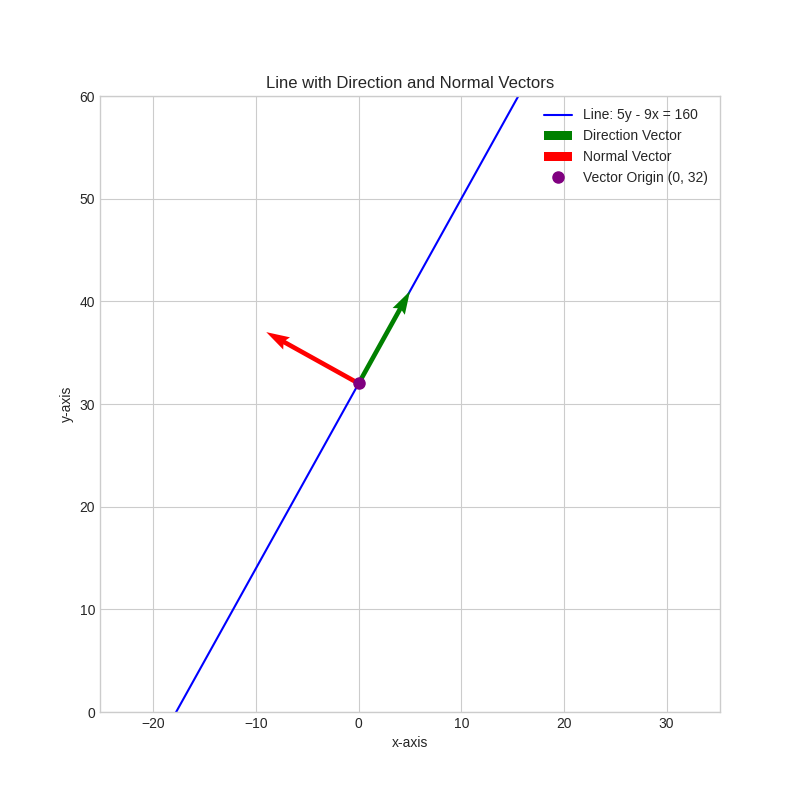
\includegraphics[width=3\columnwidth, height=0.8\textheight, keepaspectratio]{figs/fig.png}     
\end{frame}

\end{document}
